

% microtype: Tipografía.
% mathpazo: Usa la fuente Palatino.
\documentclass[a4paper, 11pt]{article}
\usepackage[protrusion=true,expansion=true]{microtype}
\usepackage{mathpazo}
\usepackage{booktabs}
\usepackage{multicol}

% Indentación de párrafos para Palatino
\setlength{\parindent}{0pt}
  \parskip=8pt
\linespread{1.05} % Change line spacing here, Palatino benefits from a slight increase by default


%%% Castellano.
% noquoting: Permite uso de comillas no españolas.
% lcroman: Permite la enumeración con numerales romanos en minúscula.
% fontenc: Usa la fuente completa para que pueda copiarse correctamente del pdf.
\usepackage[spanish,es-noquoting,es-lcroman]{babel}
\usepackage[utf8]{inputenc}
\usepackage[T1]{fontenc}
\selectlanguage{spanish}
\usepackage{graphics}
\usepackage{svg}


%%% Gráficos
\usepackage{graphicx} % Required for including pictures
\usepackage{wrapfig} % Allows in-line images



%%% Matemáticas
\usepackage{amsmath}

%%% Código

\usepackage{listings}



%%% Bibliografía
\makeatletter
\renewcommand\@biblabel[1]{\textbf{#1.}} % Change the square brackets for each bibliography item from '[1]' to '1.'
\renewcommand{\@listI}{\itemsep=0pt} % Reduce the space between items in the itemize and enumerate environments and the bibliography



%----------------------------------------------------------------------------------------
%	TÍTULO
%----------------------------------------------------------------------------------------
% Configuraciones para el título.
% El título no debe editarse aquí.
\renewcommand{\maketitle}{
  \begin{flushright} % Right align
  
  {\LARGE\@title} % Increase the font size of the title
  
  \vspace{50pt} % Some vertical space between the title and author name
  
  {\large\@author} % Author name
  \\\@date % Date
  \vspace{40pt} % Some vertical space between the author block and abstract
  \end{flushright}
}

%% Título
\title{\textbf{Práctica 1}\\ % Title
Algorítmica} % Subtitle

\author{\textsc{Fco. Javier Sáez Maldonado}\\ % Author
\textsc{Laura Gómez Garrido}\\
\textsc{Luis Antonio Ortega Andrés}\\
\textsc{Pedro Bonilla Nadal}\\
\textsc{Daniel Pozo Escalona}\vspace{2cm}
\\{\textit{Universidad de Granada}}} % Institution

\date{\today} % Date



%----------------------------------------------------------------------------------------
%	DOCUMENTO
%----------------------------------------------------------------------------------------

\begin{document}

\maketitle % Print the title section


%% Índice
{\parskip=2pt
  \tableofcontents
}
\pagebreak

%%% Inicio del documento


\section*{Introducción}

En esta primera práctica, vamos a centrarnos en el estudio de la eficiencia tanto empírica como teórica de ciertos algoritmos. Para ello, realizaremos pruebas empíricas con nuestros propios equipos para comprobar que la eficiencia empírica se ajusta de forma más o menos adecuada a la eficiencia que calcularemos de forma teórica.

Para ello, comenzaremos presentando los algoritmos que vamos a estudiar. Son algoritmos bastante conocidos y cuyas eficiencias teóricas también son conocidas. Estos son:
\begin{enumerate}
	\item Algoritmo de ordenación \textbf{burbuja}
	\item Algoritmo de ordenación por \textbf{inserción}
	\item Algoritmo de ordenación por \textbf{selección}
	\item Algoritmo de ordenación \textbf{mergesort}, basado en la técnica divide y vencerás
	\item Algoritmo de ordenación \textbf{quicksort}
	\item Algoritmo de ordenación \textbf{heapsort}
	\item Algoritmo de Floyd
	\item Algoritmo de Hanoi
\end{enumerate}

Para obtener unos buenos resultados, hemos decidido hacer las ejecuciones de estos algoritmos en varias máquinas. Las máquinas que usaremos serán:
\begin{enumerate}    
	\item Máquina A: Procesador Intel Core I7-5700HQ, 6M Cache y 3.5 Ghz.
	\item Máquina B: Procesador Intel Core I7-4712mq , 6M cache y 3.30Ghz
	\item Máquina C: Procesador: Intel Core i7-4510U ,2.00GHz
	\item Máquina D: Máquina Virtual VirtualBox version 5.1.112r112440(Qt5.6.2) dentro de una Máquina C.

\end{enumerate}

\section{Cálculo de la eficiencia empírica}
Para facilitar el cálculo de la eficiencia empírica, realizamos un script en \emph{bash} que automatizara el proceso de realizar las ejecuciones pedidas por programa y cambiara iterativamente las iteraciones de nuestros programas. El script además, compila los programas y deja los resultados en una carpeta de resultados para poder después hacer las gráficas. El código es el siguiente:

\begin{lstlisting}
mkdir resultados ejecutable 2> /dev/null

for i in *.cpp
do
    j=`echo $i | cut -f 1 -d .`
    g++ -O2 $i -o ../ejecutable/$j

    echo $j

	      echo "" > ../resultados/$j.dat
	      k="1"
	      while [ $k -le 28 ]
	      do
	          ../ejecutable/$j $k >> ../resultados/$j.dat
	          k=$[$k+1]
	      done
done

\end{lstlisting}
Además, según el tipo de algoritmo, hemos ido variando el número de veces que se ejecuta el código. El que hemos mostrado es el que ejecuta el programa de Hanoi. Los algoritmos de eficiencia $n^2$ se han ejecutado de $500$ en $500$ hasta llegar al valor de $50000$.  El algoritmo Floyd lo ejecutaremos de 25 en 25 hasta llegar a $2500$ de tamaño del vector.  Los algoritmos de eficiencie $nlogn$ los ejecutaremos de $1000$ en $1000$ hasta llegar a $100000$.

\subsection{Tablas de las ejecuciones}
Tras realizas las ejecuciones de los distintos algoritmos, los hemos agrupado por órdenes de eficiencia y hemos escrito tablas con ellos. Escribiremos  las tablas recortadas y generadas por el computador de tipo $A$, para no ocupar todo el documento con las tablas. Estas tablas podrán ser consultadas en una carpeta incluída en el proyecto.

\subsubsection{ Tablas algoritmos $n^2$}
\begin{tabular}{@{}llll@{}}
\toprule
Tamaño Vector & Burbuja  & Inserción & Selección  \\ \midrule
500           & 0.000183 & 0.00012   & 9.41e-05   \\
1000          & 0.000676 & 0.00041   & 0.00033464 \\
1500          & 0.001421 & 0.000889  & 0.00073601 \\
2000          & 0.002645 & 0.001483  & 0.00124963 \\
2500          & 0.004357 & 0.002291  & 0.002069   \\
3000          & 0.00658  & 0.003276  & 0.002789   \\
3500          & 0.009617 & 0.004485  & 0.003708   \\
4000          & 0.013066 & 0.005808  & 0.00491    \\
4500          & 0.017328 & 0.007279  & 0.006437   \\
5000          & 0.022303 & 0.00898   & 0.007507   \\
5500          & 0.0279   & 0.010837  & 0.008995   \\
6000          & 0.034061 & 0.012819  & 0.010721   \\
6500          & 0.041173 & 0.01515   & 0.012625   \\
7000          & 0.049032 & 0.017688  & 0.014594   \\
7500          & 0.057096 & 0.020175  & 0.017596   \\
8000          & 0.06641  & 0.023064  & 0.018863   \\
8500          & 0.076047 & 0.026317  & 0.02148    \\
9000          & 0.087017 & 0.029131  & 0.023866   \\
9500          & 0.099032 & 0.032499  & 0.026604   \\
10000         & 0.11069  & 0.03597   & 0.029735   \\
10500         & 0.123762 & 0.039592  & 0.032609   \\
11000         & 0.138682 & 0.043482  & 0.03555    \\
11500         & 0.151532 & 0.047382  & 0.038855   \\
12000         & 0.166319 & 0.051606  & 0.042199   \\
12500         & 0.181765 & 0.055837  & 0.045834   \\
13000         & 0.198691 & 0.060376  & 0.049303   \\
13500         & 0.21569  & 0.064976  & 0.053129   \\
14000         & 0.231813 & 0.069198  & 0.057271   \\
14500         & 0.250401 & 0.074645  & 0.061438   \\
%%%%%%%%%%%%%%%%%%%%%%%%%%%%%%%%%%%%%%%%%%%%%

15000         & 0.269076 & 0.079654  & 0.065577   \\
15500         & 0.290561 & 0.084977  & 0.069896   \\
16000         & 0.31048  & 0.090637  & 0.07443    \\
16500         & 0.330982 & 0.0963    & 0.07922    \\
17000         & 0.353309 & 0.103345  & 0.084177   \\
17500         & 0.373751 & 0.109385  & 0.09186    \\
18000         & 0.397518 & 0.115501  & 0.094513   \\
18500         & 0.426722 & 0.122327  & 0.099572   \\
19000         & 0.4511   & 0.129006  & 0.104891   \\
19500         & 0.473987 & 0.136012  & 0.11034    \\
20000         & 0.499128 & 0.143031  & 0.116565   \\
\bottomrule
\end{tabular}


Ahora, la gráfica resultante para \textbf{Burbuja} es:\\
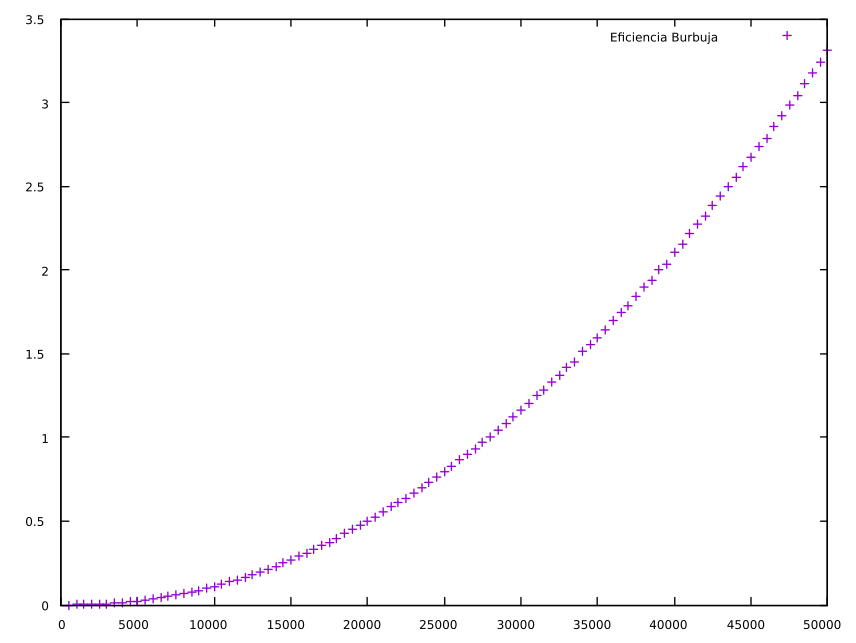
\includegraphics[scale=0.5]{pngs/Burbuja}\\
Que, ajustada al modelo conveniente ($n^2$), es:\\
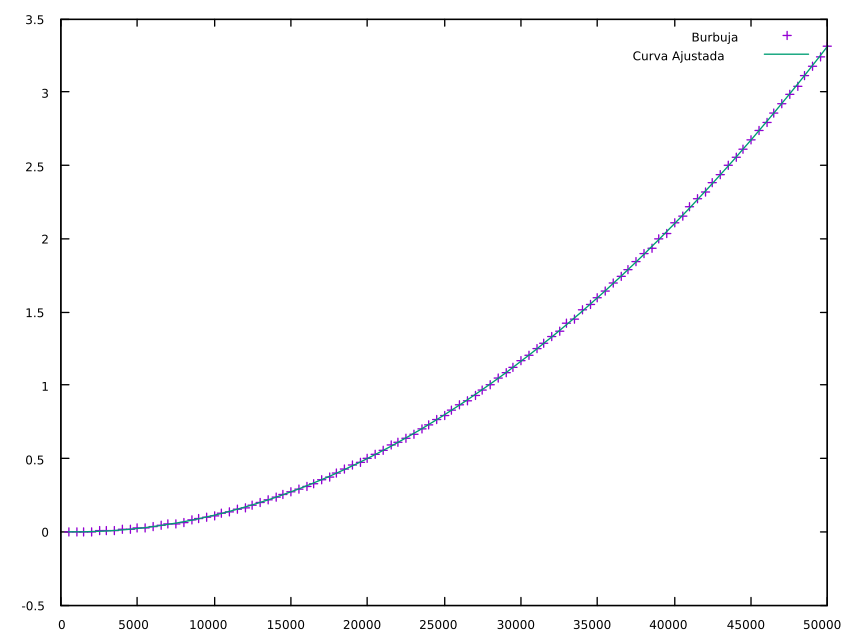
\includegraphics[scale=0.5]{pngs/BurbujaAjustada}
\newpage

La gráfica resultante para \textbf{Inserción} es:\\
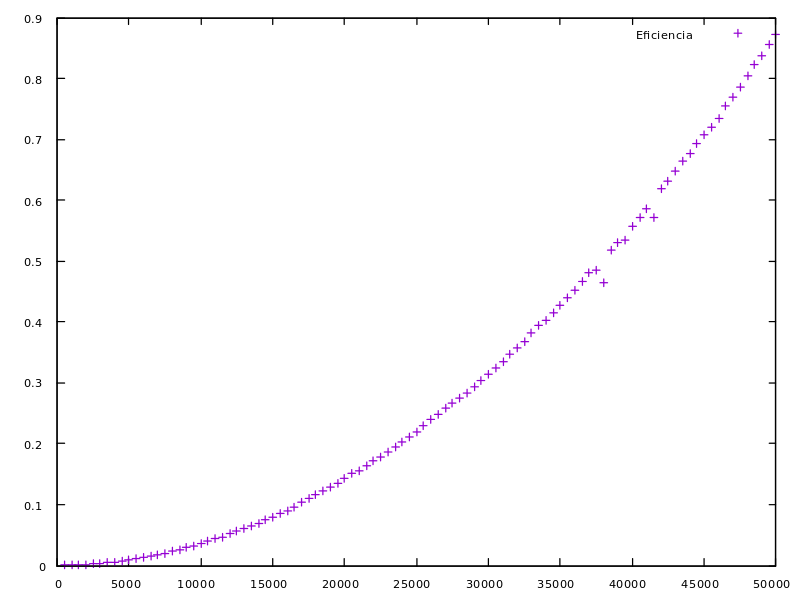
\includegraphics[scale=0.4]{pngs/Insercion}\\
Que, ajustada al modelo conveniente ($n^2$), es:\\
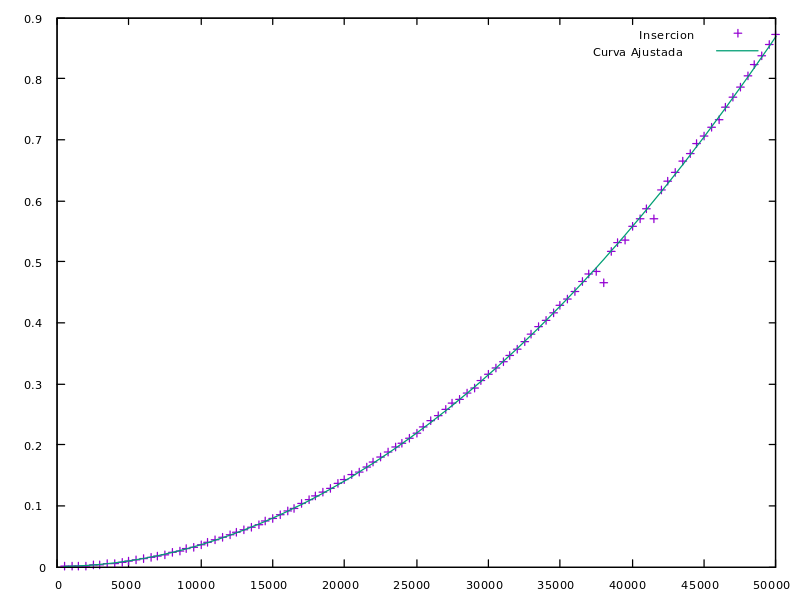
\includegraphics[scale=0.4]{pngs/InsercionAjustada}
\newpage

Por último, la gráfica resultante para \textbf{Selección} es:\\
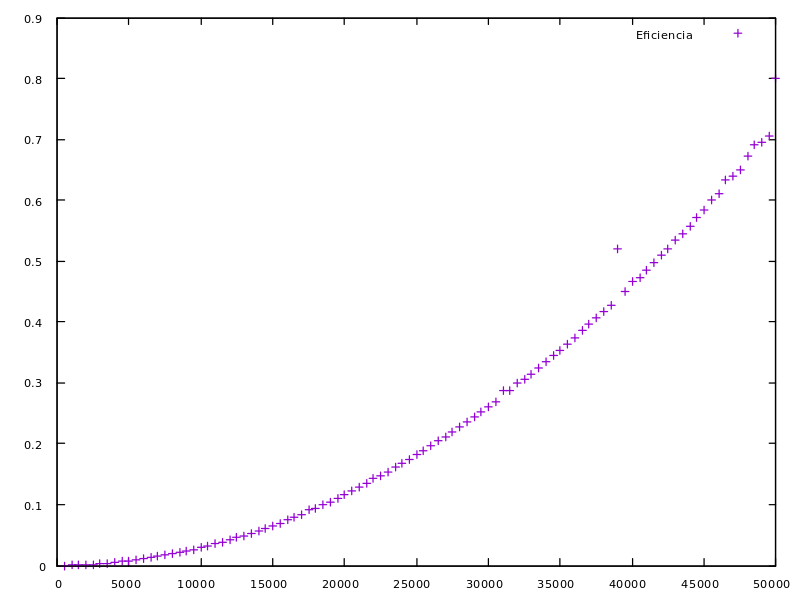
\includegraphics[scale=0.4]{pngs/Seleccion}\\
Que, ajustada al modelo conveniente ($n^2$), es:\\
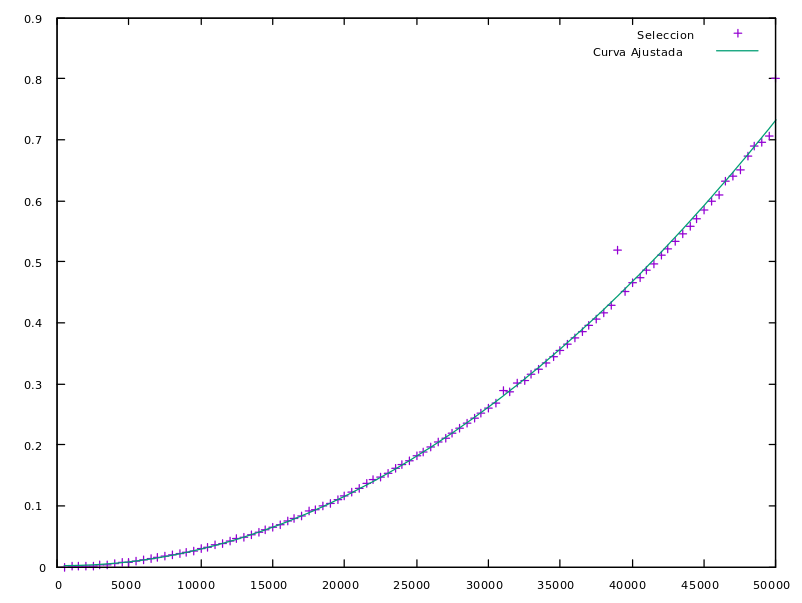
\includegraphics[scale=0.4]{pngs/SeleccionAjustada}
\newpage

Si juntamos ahora las ejecuciones en una tabla, vemos que el resultado es:\\
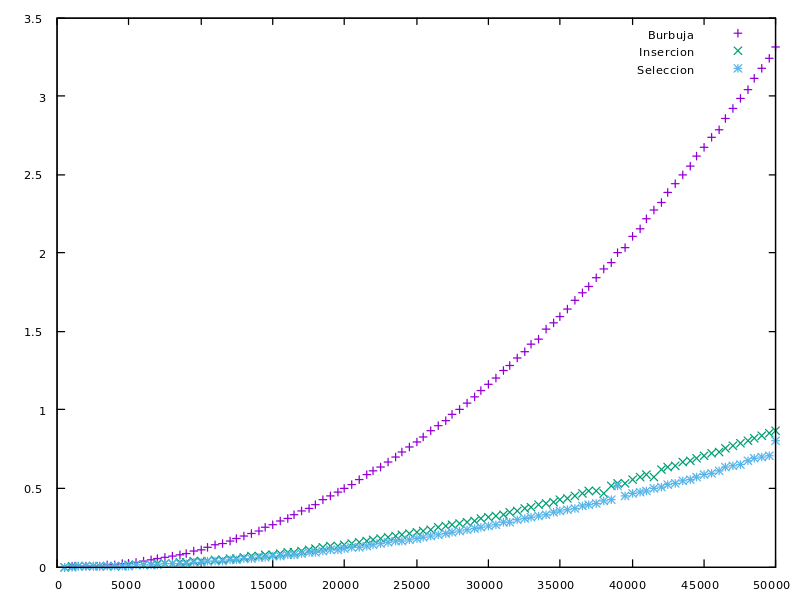
\includegraphics[scale=0.4]{pngs/Eficiencian2}

Donde se observa que burbuja tiene un grado mayor de escalabilidad con el tiempo, pero inserción y selección escalan de forma muy similar con el número de datos a tratar.

\subsubsection{Tablas algoritmos $nlogn$}
\begin{tabular}{@{}llll@{}}
\toprule
Tamaño Vector & Mergesort   & Heapsort & Quicksort \\ \midrule
1000          & 4.1423e-05  & 6.1e-05  & 4.9e-05   \\
2000          & 9.9989e-05  & 0.000142 & 9.7e-05   \\
3000          & 0.000187499 & 0.000223 & 0.00016   \\
4000          & 0.000221424 & 0.000268 & 0.000192  \\
5000          & 0.000303942 & 0.000367 & 0.000286  \\
6000          & 0.000399219 & 0.000416 & 0.000285  \\
7000          & 0.00039881  & 0.000476 & 0.000372  \\
8000          & 0.000474348 & 0.00052  & 0.00038   \\
9000          & 0.000563394 & 0.000629 & 0.000425  \\
10000         & 0.000649712 & 0.000784 & 0.000484  \\
11000         & 0.000845    & 0.000783 & 0.000528  \\
12000         & 0.000895    & 0.000903 & 0.000607  \\
13000         & 0.000838    & 0.000944 & 0.000659  \\
14000         & 0.000898    & 0.001027 & 0.000732  \\
15000         & 0.000968    & 0.001096 & 0.000847  \\
16000         & 0.001065    & 0.001107 & 0.000836  \\
17000         & 0.00123     & 0.001167 & 0.000906  \\
18000         & 0.001332    & 0.001311 & 0.001203  \\
19000         & 0.001334    & 0.001318 & 0.000972  \\
20000         & 0.001487    & 0.001464 & 0.00107   \\
21000         & 0.001621    & 0.00148  & 0.001146  \\
22000         & 0.001656    & 0.001573 & 0.001186  \\
23000         & 0.001772    & 0.00167  & 0.001244  \\
24000         & 0.001905    & 0.001867 & 0.001324  \\
25000         & 0.002049    & 0.00199  & 0.001348  \\
26000         & 0.001807    & 0.001893 & 0.001459  \\
27000         & 0.001879    & 0.00198  & 0.00151   \\
28000         & 0.001937    & 0.002086 & 0.001498  \\
29000         & 0.002007    & 0.00212  & 0.001579  \\
30000         & 0.002077    & 0.002397 & 0.001664  \\
31000         & 0.002285    & 0.002336 & 0.001741  \\
32000         & 0.002266    & 0.002378 & 0.001808  \\
33000         & 0.00244     & 0.002577 & 0.001808  \\
34000         & 0.002571    & 0.002529 & 0.00185   \\
35000         & 0.002595    & 0.002641 & 0.001948  \\
36000         & 0.002639    & 0.002733 & 0.002045  \\
37000         & 0.002763    & 0.002752 & 0.002108  \\
38000         & 0.002913    & 0.002832 & 0.002109  \\
39000         & 0.002961    & 0.002919 & 0.002195  \\
40000         & 0.003039    & 0.003069 & 0.002246  \\\bottomrule
\end{tabular}

Ahora, la gráfica resultante para \textbf{Mergesort} es:\\
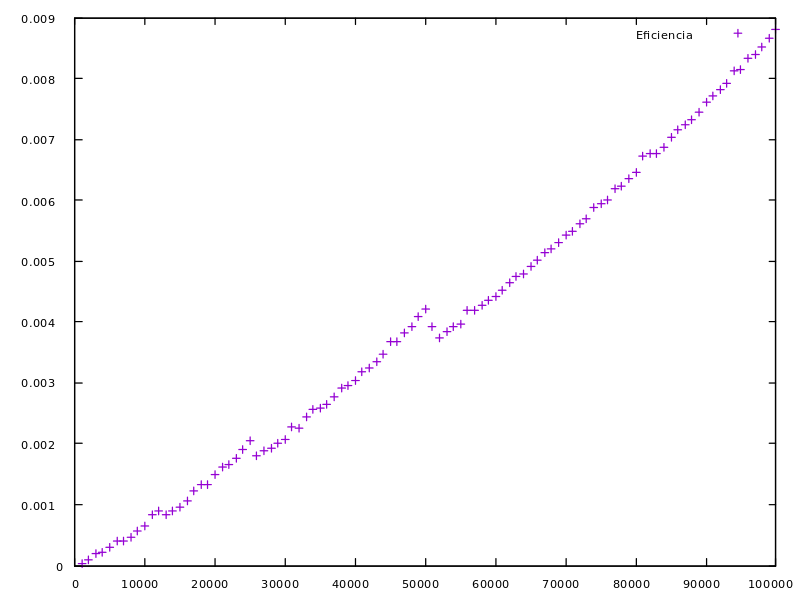
\includegraphics[scale=0.4]{pngs/Mergesort}\\
Que, ajustada al modelo conveniente ($nlogn$), es:\\
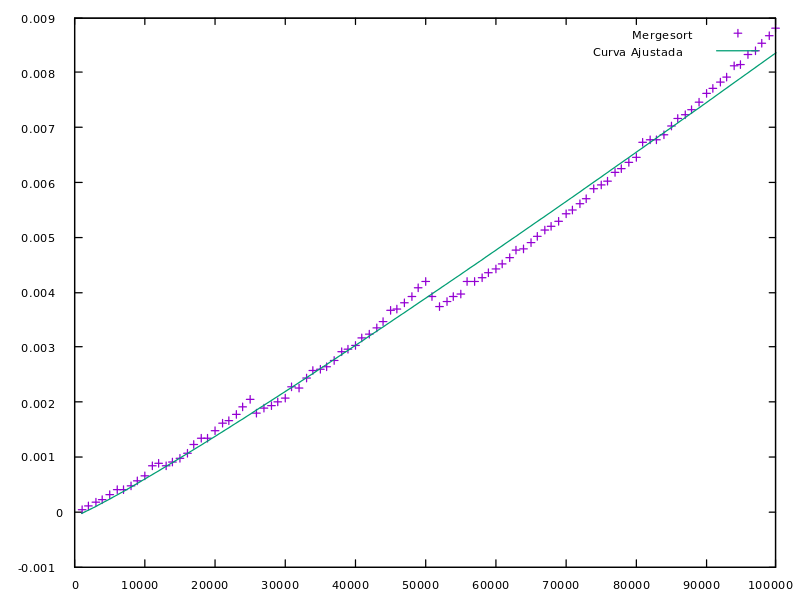
\includegraphics[scale=0.4]{pngs/MergesortAjustada}
\newpage


La gráfica resultante para \textbf{Heapsort} es:\\
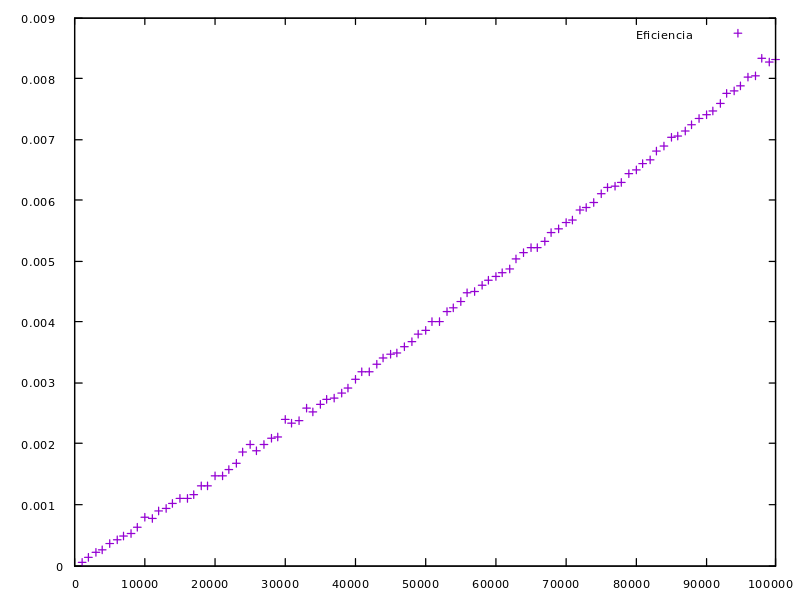
\includegraphics[scale=0.4]{pngs/Heapsort}\\
Que, ajustada al modelo conveniente ($nlogn$), es:\\
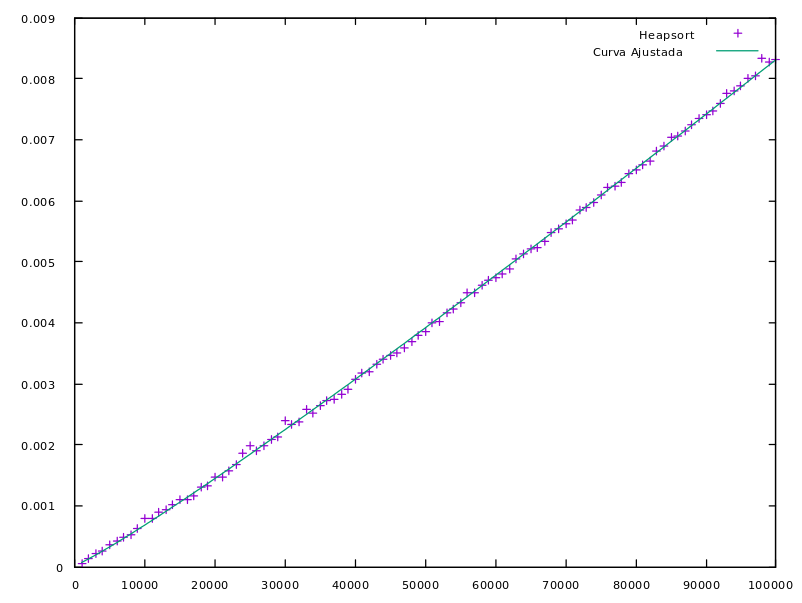
\includegraphics[scale=0.4]{pngs/HeapsortAjustada}
\newpage

Por último dentro de este bloque, la gráfica resultante para \textbf{Quicksort} es:\\
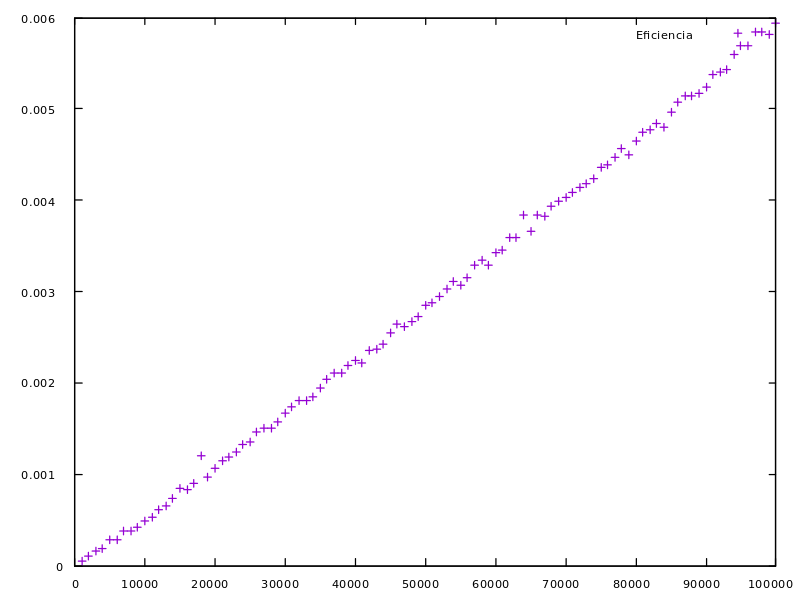
\includegraphics[scale=0.4]{pngs/Quicksort}\\
Que, ajustada al modelo conveniente ($nlogn$), es:\\
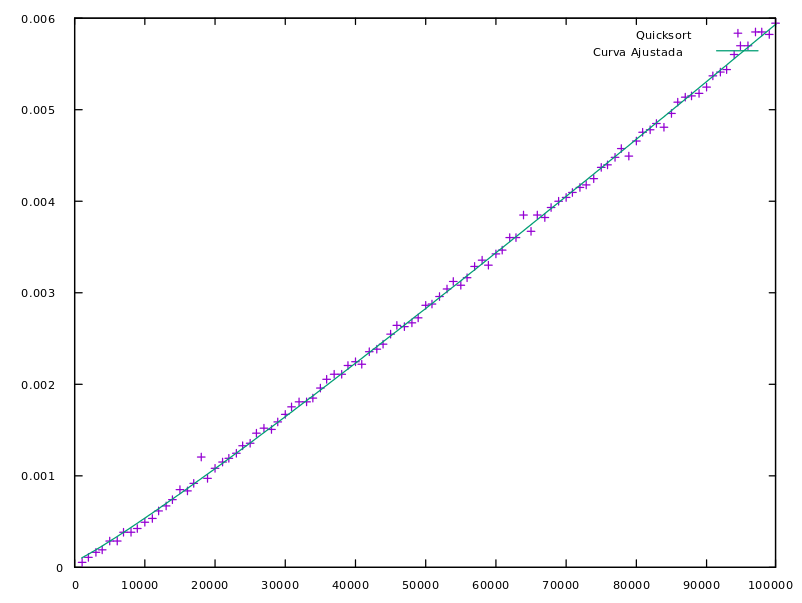
\includegraphics[scale=0.4]{pngs/QuicksortAjustada}
\newpage

Estos tres algoritmos son comparables en eficiencia en la siguiente gráfica:
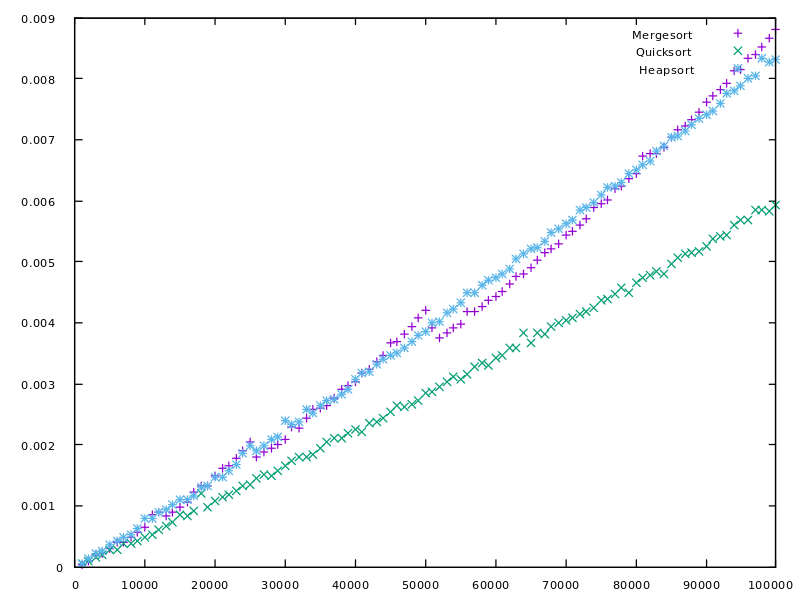
\includegraphics[scale=0.4]{pngs/nlogn}

Donde podemos comprobar que tienen comportamientos de eficiencia muy similares.


\subsubsection{Comparativa ordenación}


Habiendo terminado el bloque de algoritmos de ordenación, podemos establecer una comparativa entre ellos con la siguiente gráfica:\\
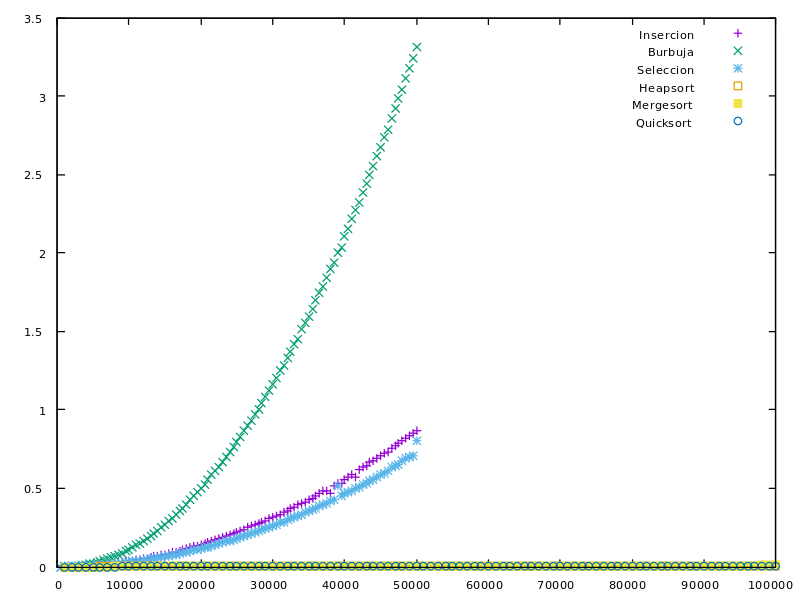
\includegraphics[scale=0.5]{pngs/Ordenacion}
\subsubsection{Tabla algoritmo Hanoi}


\begin{tabular}{@{}ll@{}}
\toprule
Tamaño Vector & Hanoi    \\ \midrule
1             & 1,00E-06 \\
2             & 1,00E-06 \\
3             & 1,00E-06 \\
4             & 1,00E-06 \\
5             & 1,00E-06 \\
6             & 1,00E-06 \\
7             & 1,00E-06 \\
8             & 2,00E-06 \\
9             & 2,00E-06 \\
10            & 4,00E-06 \\
11            & 6,00E-06 \\
12            & 1.1e-05  \\
13            & 1.8e-05  \\
14            & 3.8e-05  \\
15            & 8.2e-05  \\
16            & 0.000174 \\
17            & 0.000324 \\
18            & 0.000663 \\
19            & 0.001226 \\
20            & 0.002177 \\
21            & 0.004413 \\
22            & 0.008785 \\
23            & 0.017613 \\
24            & 0.034917 \\
25            & 0.069979 \\
26            & 0.138508 \\
27            & 0.276828 \\
28            & 0.552919 \\ \bottomrule
\end{tabular}
\newpage

De estos datos, podemos obtener la gráfica del algoritmo de \textbf{Hanoi} siguiente:\\
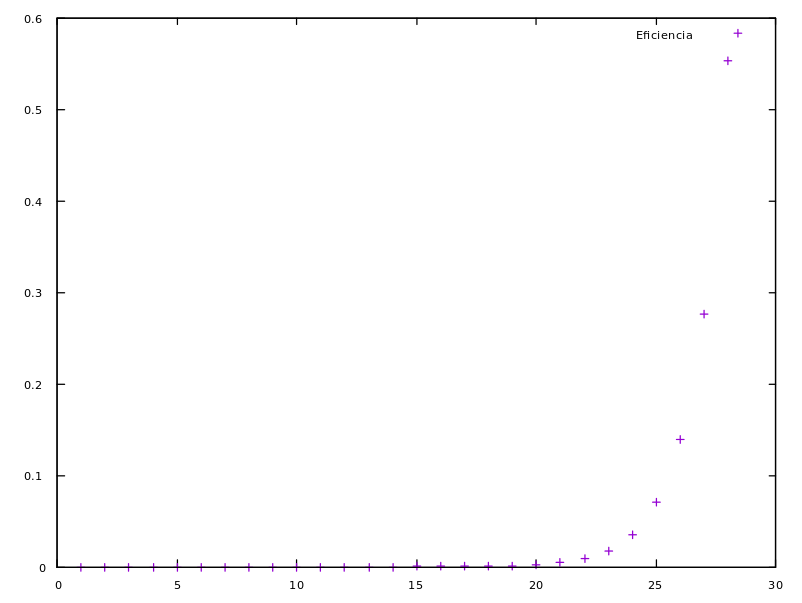
\includegraphics[scale=0.4]{pngs/Hanoi}\\
Que, ajustada a su modelo $2^n$, da como resultado la gráfica:\\
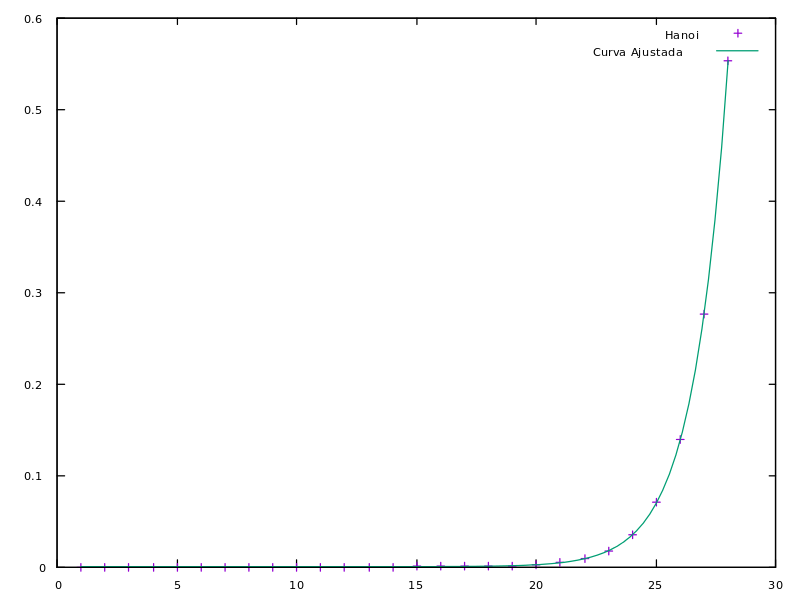
\includegraphics[scale=0.4]{pngs/HanoiAjustada}

Esta puede parecer distinta a una gráfica de una función $2^n$, pero sin embargo esto ocurre por el bajo rango de sus datos, pues la escalabilidad en tiempo de esta función es demasiado alta y no se podría mantener unos datos mucho más altos si queremos que el programa se ejecute en un tiempo razonable.

\subsubsection{Tabla algoritmo Floyd}
\begin{tabular}{@{}ll@{}}
\toprule
Tamaño Vector & Floyd    \\ \midrule
50            & 0.000147 \\
75            & 0.000422 \\
100           & 0.000841 \\
125           & 0.001555 \\
150           & 0.002624 \\
175           & 0.004146 \\
200           & 0.005986 \\
225           & 0.008689 \\
250           & 0.011423 \\ 
275           & 0.015214 \\
300           & 0.019555 \\
325           & 0.024801 \\
350           & 0.030623 \\
375           & 0.037862 \\
400           & 0.045488 \\
425           & 0.058492 \\
450           & 0.069071 \\
475           & 0.079011 \\
500           & 0.08839  \\
525           & 0.102404 \\
550           & 0.119307 \\
575           & 0.134324 \\
600           & 0.161119 \\
625           & 0.172804 \\
650           & 0.192393 \\
675           & 0.216992 \\
700           & 0.240593 \\
725           & 0.269456 \\
750           & 0.295816 \\
775           & 0.327231 \\
800           & 0.359917 \\
825           & 0.408639 \\
850           & 0.433239 \\
875           & 0.47942  \\
900           & 0.522784 \\
925           & 0.577851 \\
950           & 0.618519 \\
975           & 0.675189 \\
1000          & 0.759402 \\ \bottomrule
\end{tabular}

De estos datos, podemos obtener la gráfica del algoritmo de \textbf{Floyd} siguiente:\\
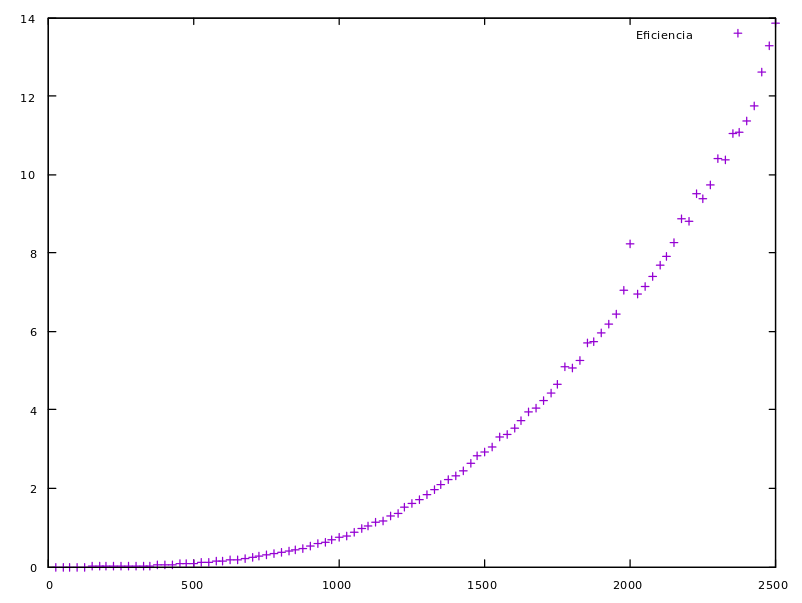
\includegraphics[scale=0.4]{pngs/Floyd}\\
Que, ajustada a su modelo $2^n$, da como resultado la gráfica:\\
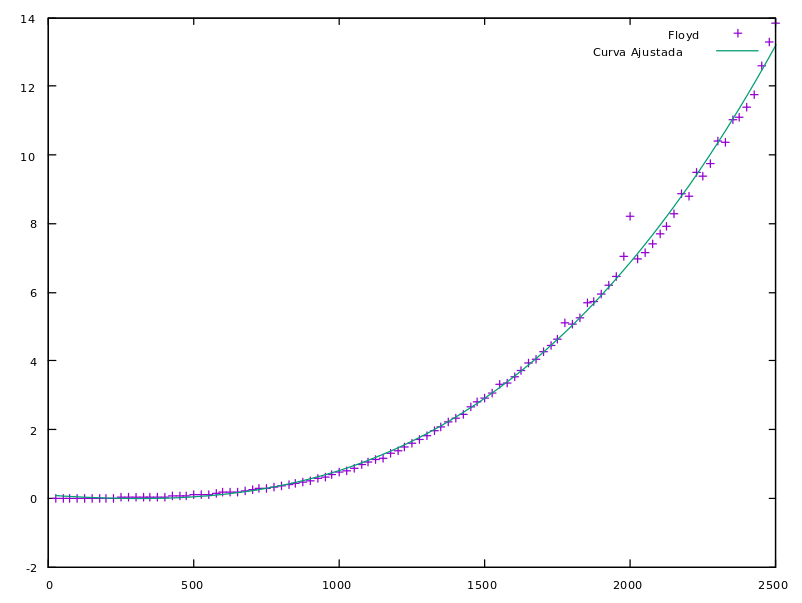
\includegraphics[scale=0.4]{pngs/FloydAjustada}

Donde podemos comprobar que los resultados obtenidos, salvo ruido, se ajustan bien a los teóricos.

\end{document}